\documentclass[oneside,11pt,a4paper]{article}

% PACKAGES %

\usepackage[utf8]{inputenc}    
\usepackage[T1]{fontenc}
\usepackage[francais]{babel}
\usepackage{graphicx}
\usepackage{layout}
\usepackage{lipsum}
\usepackage{tikz}
\usepackage{lscape}
\usepackage{listings}
\usepackage{amsmath}
\usepackage{amssymb}
\usepackage{placeins}
\usepackage{array}
%\usepackage[active,tightpage]{preview}

% D�fini les marges � 2 cm
\usepackage[top=1cm, bottom=2cm, left=2.5cm, right=2.5cm]{geometry}

% Supprime l'indentation de la premi�re ligne des paragraphes
\setlength{\parindent}{0pt}
\setlength{\parskip}{10pt}

% DOCUMENT %

\begin{document}
\title{Database project - deliverable 1}
\author{
	Valentin \bsc{Matter}\\\small{203447}
	\and
	Colla \bsc{Rensch}\\\small{205814}
	\and
	Arthur \bsc{Giroux}\\\small{205443}
}
\date{March $^{24th}$ 2013} 

\maketitle

\section{ER model}

\begin{center}
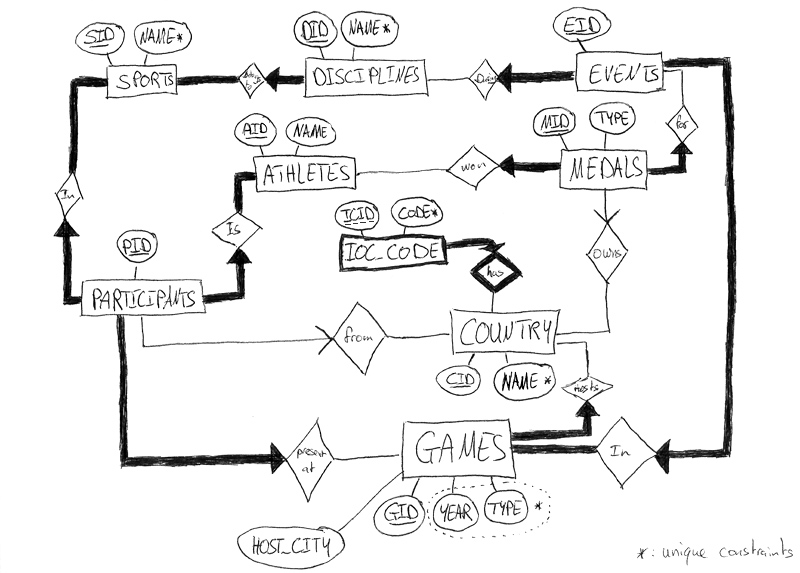
\includegraphics[height=310px]{ermodel.jpg}
\end{center}

\noindent\hrulefill

\section{Tables creation}


\noindent\hrulefill

\section{Remarks}

\begin{itemize}
	\item athlete X
	\item countries, sports, disciplines, events, games : unique name
	\item medal - country
	\item games - number\_of\_countries, number\_of\_athletes, number\_of\_events
	\item contraintes ?
\end{itemize}

\noindent\hrulefill

\end{document}